
\documentclass[hide notes,intlimits]{beamer}


\mode<presentation>
{
  \usetheme[headline,footline]{UAFshade}
  \setbeamercovered{transparent}
}

% load packages
\usepackage[english]{babel}
\usepackage[latin1]{inputenc}
\usepackage[T1]{fontenc}
\usepackage{multimedia,pgf}
\usepackage{lmodern}
\usepackage[amssymb]{SIunits}
\usepackage{hyperref}
\usepackage{natbib}
\bibliographystyle{andy}


% title page
\title[Glacier Dynamics] % (optional, use only with long paper titles)
{Thermodynamics of Glaciers}
\subtitle{Glaciers 617}


\author[Aschwanden] % (optional, use only with lots of authors)
{Andy Aschwanden}
% - Give the names in the same order as the appear in the paper.
% - Use the \inst{?} command only if the authors have different
%   affiliation.

\institute[ARSC] % (optional, but mostly needed)
{
  %
  Arctic Region Supercomputing Center\\
  University of Alaska Fairbanks, USA
}
% - Use the \inst command only if there are several affiliations.
% - Keep it simple, no one is interested in your street address.

\titlegraphic{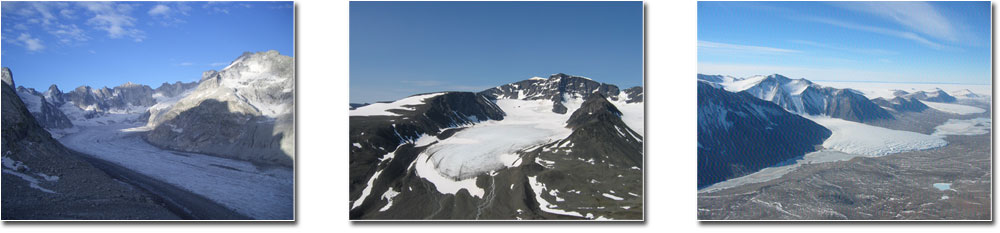
\includegraphics[width=10cm]{images/glaciers3}}


\subject{Glaciers}

% define what is shown at the beginning of each section
\AtBeginSection[]
{
 \begin{frame}<beamer>
   \frametitle{Outline}
   \tableofcontents[currentsection,subsectionstyle=hide/hide/hide]
 \end{frame}
}

% define what is shown at the beginning of each subsection
% \AtBeginSubsection[]
% {
%  \begin{frame}<beamer>
%   \frametitle{Outline}
%    \tableofcontents[currentsection,currentsubsection]
%  \end{frame}
% }

\begin{document}

% insert titlepage
\begin{frame}
  \titlepage
\end{frame}

% insert TOC
\begin{frame}
 \frametitle{Outline}
 \tableofcontents[subsectionstyle=hide]
  %You might wish to add the option [pausesections]
\end{frame}


\section{Introduction}


\begin{frame}
  \begin{figure}
    \includegraphics<1>[width=11cm]{images/glacier_opaque}%
    \includegraphics<2>[width=11cm]{images/glacier_temp}%
    \includegraphics<3>[width=11cm]{images/glacier_poly}%
    \includegraphics<4>[width=11cm]{images/glacier_cold}%    
  \end{figure}
  \begin{overlayarea}{4cm}{.5cm}
  \only<2>{\small Photo: A. Aschwanden}
  \only<3>{\small Photo: R. Hock}
  \only<4>{\small Photo: S. White}  
  \end{overlayarea}
  \note<1>{
  \begin{itemize}
  \item before bothering you with nasty equations and physics, start off with three pictures
  \end{itemize}
  }   
  \note<2>{Fornogletscher, Switzerland}
  \note<3>{Storglaci\"aren, northern Sweden}
  \note<4>{Canada Glacier, Dry Valleys, Antarctica}
\end{frame}




\subsection{Types of Glaciers}

\begin{frame}
\frametitle{Types of Glaciers}
\begin{columns}
  \column[C]{4cm}
  \begin{figure}
    \includegraphics<1>[width=2.35cm]{images/taylor_valley_w}
  \end{figure}      
  \column[C]{8.5cm}
  \begin{block}
  {cold glacier} ice below pressure melting point, no liquid water
  \end{block}
\end{columns}
\begin{columns}
  \column[C]{4cm}
  \begin{figure}
    \includegraphics<1>[width=2.35cm]{images/forno_w}%
  \end{figure}
  \column[C]{8.5cm}
  \begin{block}
  {temperate glacier} ice at pressure melting point, contains liquid water in the ice matrix
  \end{block}
\end{columns}
\begin{columns}
  \column[C]{4cm}
  \begin{figure}
    \includegraphics<1>[width=2.35cm]{images/stor_w}
  \end{figure}     
  \column[C]{8.5cm}
  \begin{block}
  {polythermal glacier} cold and temperate parts
  \end{block}
\end{columns}
  \note{
  \begin{itemize}
  \item these 3 glaciers serve as examples of 3 glacier types
  \end{itemize}
  }   
\end{frame}


\subsection{Glacier Physics}

\begin{frame}
  \frametitle{Glacier Ice}
  \begin{itemize}
    \item incompressible, heat-conducting, strain-softening fluid
    \item quasi-stationary flow (Reynolds number $\le 10^{-10}$)
  \end{itemize}
  The \alert{viscosity} of ice depends on
  \begin{itemize}
    \item<1> temperature (cold ice) $\Rightarrow$ well established
    \item<1> water content (temperate ice) $\Rightarrow$ poorly known
    \item<1> effective strain rate
    \item<1> impurities, crystal size and crystal orientation
  \end{itemize}
  \note<1>{
  \begin{itemize}
  \item important for the thermodynamics of glaciers is the viscosity...
  \end{itemize}
  }   
\end{frame}


\begin{frame}
  \frametitle{Definition of Enthalpy}
  \begin{itemize}
  \item A new variable in ice sheet modeling
  \item Enthalpy is often used in association with phase changes
  \item \alert{Specific enthalpy ${H}$} is generally defined in thermodynamics as
    \begin{displaymath}
      {H} = u + p/\rho
    \end{displaymath}
  \item For incompressible fluids we have  
    \begin{displaymath}
      {H} = u
    \end{displaymath}
  \end{itemize}
  where 
  \begin{center}
    \begin{tabular}{cl}
      $u$ & specific inner energy\\
      $p$ & pressure\\
      $\rho$ & density
    \end{tabular}
  \end{center}
\end{frame}



\begin{frame}
  \frametitle{Cold Ice}
  \begin{columns}
    \column[c]{4cm} 
    \hspace{2em}{\includegraphics<1>[width=2.35cm]{images/glaciersv_c}}%
    \column[c]{8cm}
    \begin{block}{Definition} 
      \begin{equation*}
        \label{eq:enthalpy-cold}
        \delta H = c\,\delta T, \qquad  \omega = 0
      \end{equation*}
    \end{block}
    \begin{block}{Fourier-type sensible heat flux}
      \begin{equation*}
        \label{eq:enthalpy-flux-cold}
        {\bf q}  = {\bf q}_{s} = -k\nabla T
      \end{equation*}
    \end{block}
    \begin{block}{Temperature equation}
      \begin{equation*}
        \label{eq:cold_pde}
        \rho c\left(\frac{\partial T}{\partial t} + {\bf v}\cdot\nabla T\right) =  - \nabla \cdot {\bf q} + Q
      \end{equation*}
    \end{block}
  \end{columns}  
  \note<1>{
    \begin{itemize}
    \item ice is defined as cold, if a change in enthalpy $H$ leads to a change in temperature $T$ alone
    \item $c$ is the heat capacity of ice
    \item cold ice is free of liquid water
    \item heat flux ${\bf q}$ is  a sensible heat flux ${\bf q}_{\sf s}$ described by the Fourier equation, where $k$ is the thermal conductivity
    \item put all together, we get an equation which describes the temperature distribution and evolution in cold ice
    \item advection-dominated transport, thermomechanically-coupled problem
    \item velocity field required
    \end{itemize}
  }
\end{frame}



\begin{frame}
  \frametitle{Temperate Ice}
  \begin{columns}
    \column[c]{4cm} 
    \hspace{2em}{\includegraphics<1>[width=2.35cm]{images/glaciersv_t}}%
    \column[c]{8cm}
    \begin{block}{Definition} 
      \begin{equation*}
        \label{eq:enthalpy-temperate}
        \delta H = L\,\delta \omega, \qquad  
        \begin{array}{l}
          T = T_{m} \\[.2em]
          \omega = \frac{m_{\sf w}}{m_{\sf w}+m_{\sf i}}
        \end{array}
      \end{equation*}
    \end{block}
    \begin{block}{Latent heat flux}
      \begin{equation*}
        \label{eq:enthalpy-flux-temperate}
        {\bf q}  = {\bf q}_{l} =
        \left\{
          \begin{array}{ll}
            -L\nu \nabla \omega & \textsf{Fick-type}  \\
            L\omega {\bf v}_{j} & \textsf{Darcy-type} 
          \end{array}
        \right.
      \end{equation*}
    \end{block}
    \begin{block}{Water content equation}
      \begin{equation*}
        \label{eq:temperate_pde}
        \rho L\left(\frac{\partial \omega}{\partial t} + {\bf v}\cdot\nabla \omega\right)  = -\nabla \cdot {\bf q} + Q
      \end{equation*}
    \end{block}
  \end{columns}    
  \note<1>{
    \begin{itemize}
    \item ice is defined as temperate, if a change in enthalpy $H$ leads to a change in water content $\omega$ alone
    \item $L$ is the latent heat of fusion
    \item temperate ice contains a small amount of liquid water, $\omega$, which is defined as the mass fraction of liquid water in the ice-water mixture
    \item little is known about the nature of the latent heat flux ${\bf q}_{l}$
    \item Fick-type and Darcy-type diffusion were proposed
    \item however, not enough lab and field experiments available to further constrain the latent heat flux
    \item assumed to be small
    \item put all together, we get an equation which describes the water content distribution and evolution in temperate ice
    \item strongly advection-dominated transport, thermomechanically-coupled problem
    \end{itemize}
  }
\end{frame}

\begin{frame}
  \frametitle{Polythermal Glaciers}
  \begin{columns}
    \column[c]{4cm} 
    \hspace{2em}{\includegraphics<1>[width=2.35cm]{images/glaciersv_p}}%
    \column[c]{8cm}
    \begin{itemize}
    \item contains both cold and temperate ice
    \item separated by the cold-temperate transition surface (CTS)
    \item CTS is an internal free surface of discontinuity where phase changes may occur
    \end{itemize}
  \end{columns}   
\end{frame}




\subsection{Thermal Structures}

\begin{frame}
  \frametitle{Thermal Structures}
  \begin{figure}
    \includegraphics<1>[width=10.5cm]{figures/CTSstructures_allcol}
    \includegraphics<2>[width=10.5cm]{figures/CTSstructures_aecol}
    \\ \footnotesize Courtesy of R.~Pettersson
  \end{figure}
  \note{
    \begin{itemize}
    \item besides fully cold and temperate glaciers, 6 different thermal structures have been identified
    \item whereof a) and e) are the most relevant ones
    \item a) Canadian-type polythermal glacier. Bulk of ice is cold, but a temperate basal layer exists due to meltwater production resulting from strain heating
    \item e) Scandinavian-type polythermal glacier. Bulk of ice is temperate except a near-surface cold layer in the ablation zone.
    \end{itemize}
  }
\end{frame}





\section{Mathematical Model}

\begin{frame}
  \frametitle{Enthalpy Methods}
  \begin{block}{Idea}
    Solve enthalpy equation directly
    \begin{equation*}
      \rho \dot H = - \nabla \cdot {\bf q} + Q
    \end{equation*}
    similar to
    \begin{equation*}
      \rho c \dot T = - \nabla \cdot {\bf q}_{s} + Q
    \end{equation*}
    \begin{itemize}
    \item easy to implement
    \item works on fixed-grid, no front-tracking required
    \item same type of PDE as temperature equation in ``cold-ice method'' ice sheet models
    \item[$\Rightarrow$] same solvers can be used
    \end{itemize}
  \end{block}	
\end{frame}


  \begin{frame}
  \frametitle{Enthalpy, Temperature and Moisture Content}
  \vspace{-.5em}
  \begin{columns}  
  \column{8cm}
  \begin{figure}
    \includegraphics<1>[width=8cm]{figures/phase_change}
  \end{figure} \vspace{-.8em}
  \small
   $H_{\sf s}$: enthalpy of solid ice \quad @ $T=T_{\sf m},\; \omega = 0$ \\
   $H_{\sf l}$: enthalpy of liquid water @ $T=T_{\sf m},\; \omega = 1$ \\
   $T' = T - T_{m}$: temperature relative to $T_{\sf m}$  
  \column{4cm}
  \small
  \alert{cold ice}\\[.3em]
  $T  =  \frac{1}{c}\left(H-H_{\sf s}\right) + T_{\sf m}$ \\[.2em]
  $\omega  =  0$ \\[.6em]
  \alert{CTS} \\[.3em]
  $T  =  T_{\sf m}$ \\[.2em]
  $\omega  =  0$ \\[.6em]
  \alert{temperate ice}  \\[.3em]
  $T  = T_{\sf m} $ \\[.2em]
  $\omega  =   \frac{1}{L}\left(H-H_{\sf s}\right)$ \\[.6em]
  \alert{liquid water} \\[.3em]
  $T  =  \frac{1}{c}\left(H+H_{\sf l}\right) + T_{\sf m} $ \\[.2em]
  $\omega  =  1$
  \end{columns}
  \note{
  \begin{itemize}
  \item this plot illustrates the Enthalpy Method
  \item corresponding mathematical formulations on the right side
  \item $H_{\sf s}$ is the enthalpy of solid ice at the pressure melting point and zero liquid water content
  \item $H_{\sf l}$ is the enthalpy of liquid water at the pressure melting point
  \item $T$ prime is the temperature relative to the pressure melting point
  \item enthalpy on the horizontal axis
  \item temperature $T$ prime (solid line) and moisture content $\omega$ (dashed line)
  \item  
  \end{itemize}
  }
\end{frame}


\begin{frame}
  \frametitle{Enthalpy Gradient Method (EGM)}
  \begin{block}{Idea}
  \begin{itemize}
  \item assume gradient-driven diffusion (Fourier's law in cold ice, Fick-diffusion in temperate ice)
  \item differentiate the definitions for cold and temperate ice 
  \item express energy flux, ${\bf q}$, in terms of the gradient of enthalpy, $\nabla H$
   \end{itemize}
  \begin{equation*}
  {\bf q} = -\rho\kappa\nabla H
  \end{equation*}
  \begin{itemize}
  \item define the ``enthalpy diffusivity'', $\kappa$:
  \begin{equation*}
   \kappa =  \left\{
      \begin{array}{cl}
      \frac{k}{\rho c}  & \textsf{cold ice}  \vspace{.5em} \\
      \frac{\nu}{\rho} & \textsf{temperate ice}
      \end{array}
      \right.
  \end{equation*}
  \end{itemize} 
  \end{block}	
\end{frame}

\end{document}
